\chapter{\emph{Data Warehouse}}

%

Como o nome sugere, \emph{Data Warehouse} (DW), em português, significa armazém de dados. Segundo Inmon (\citeyear{inmon2002}) um \emph{Data Warehouse} é uma coleção de dados de uma coorporação que tem como objetivo dar suporte a tomada de decisão.

%

O DW tem como caracteristica ser:

%

\begin{itemize}
\item \textbf{Integrado}: capaz de integrar dados de diversas fontes de formatos.
\item \textbf{Orientado a assunto}: um sistema corporativo pode fornecer diversas informações sobre determinados aspectos da corporação. O DW é construído focando em alguns aspectos específicos, como por exemplo, em um sistema de vendas de uma loja, podemos analisar as informações sobre venda, como também podemos analisar informações sobre frequência de funcionários ou também sobre o estoque. Cada aspecto sugere a seleção de apenas dados específicos do sistema que serão uteis para a análise desse aspecto. Os demais dados não são de interesse.
\item \textbf{Não volátil}: os dados de um DW representam a informação capturada em um determinado momento da aplicação. Em aplicações, os dados estão sempre sujeitos a modificações. Dessa forma, o DW irá capturar novamente, em outro momento, essa informação e irá acrescentá-la, e não atualiza-la, ao DW, permitindo visualizar a atualização dessa determinada informação em momentos diferentes. Ou seja, os dados de um DW não são modificados, salvo raras excessões.
\item \textbf{Temporais}: consiste em armazenar a data referente à informação ou à coleta da informação. Dessa forma, o DW consegue fornecer várias visões da informação agrupadas por medidas de tempo. 
\end{itemize}

\section{\emph{Data Warehousing}}

O conjunto de ferramentas de manipulação dos dados, desde sua extração até a sua visualização para o apoio a consultas e tomada de decisão é denominado de \emph{Data Warehousing} (DWing). Portanto,  DWing não são as tecnologias em si envolvidas e sim uma arquitetura que requer o suporte de diferentes tipos de tecnologias \cite{inmon2002}.  As principais tecnologias envolvidas em um ambiente de DWing são:

%

\begin{itemize}
\item SGBDS – Gerenciadores de bases de dados
\item Sistemas de conversão e transformação de dados (ferramentas de ETL)
\item Tecnologias cliente e servidor para dar acesso aos dados a múltiplos clientes
\item Ferramentas de análise e geração de relatórios.
\end{itemize}

%

Kimball (\citeyear{kimball2002}) define os componentes básicos de um ambiente de dwing da seguinte forma:

IMAGEM dos componente KIMBAL
\begin{figure}[!htb]
	\centering
		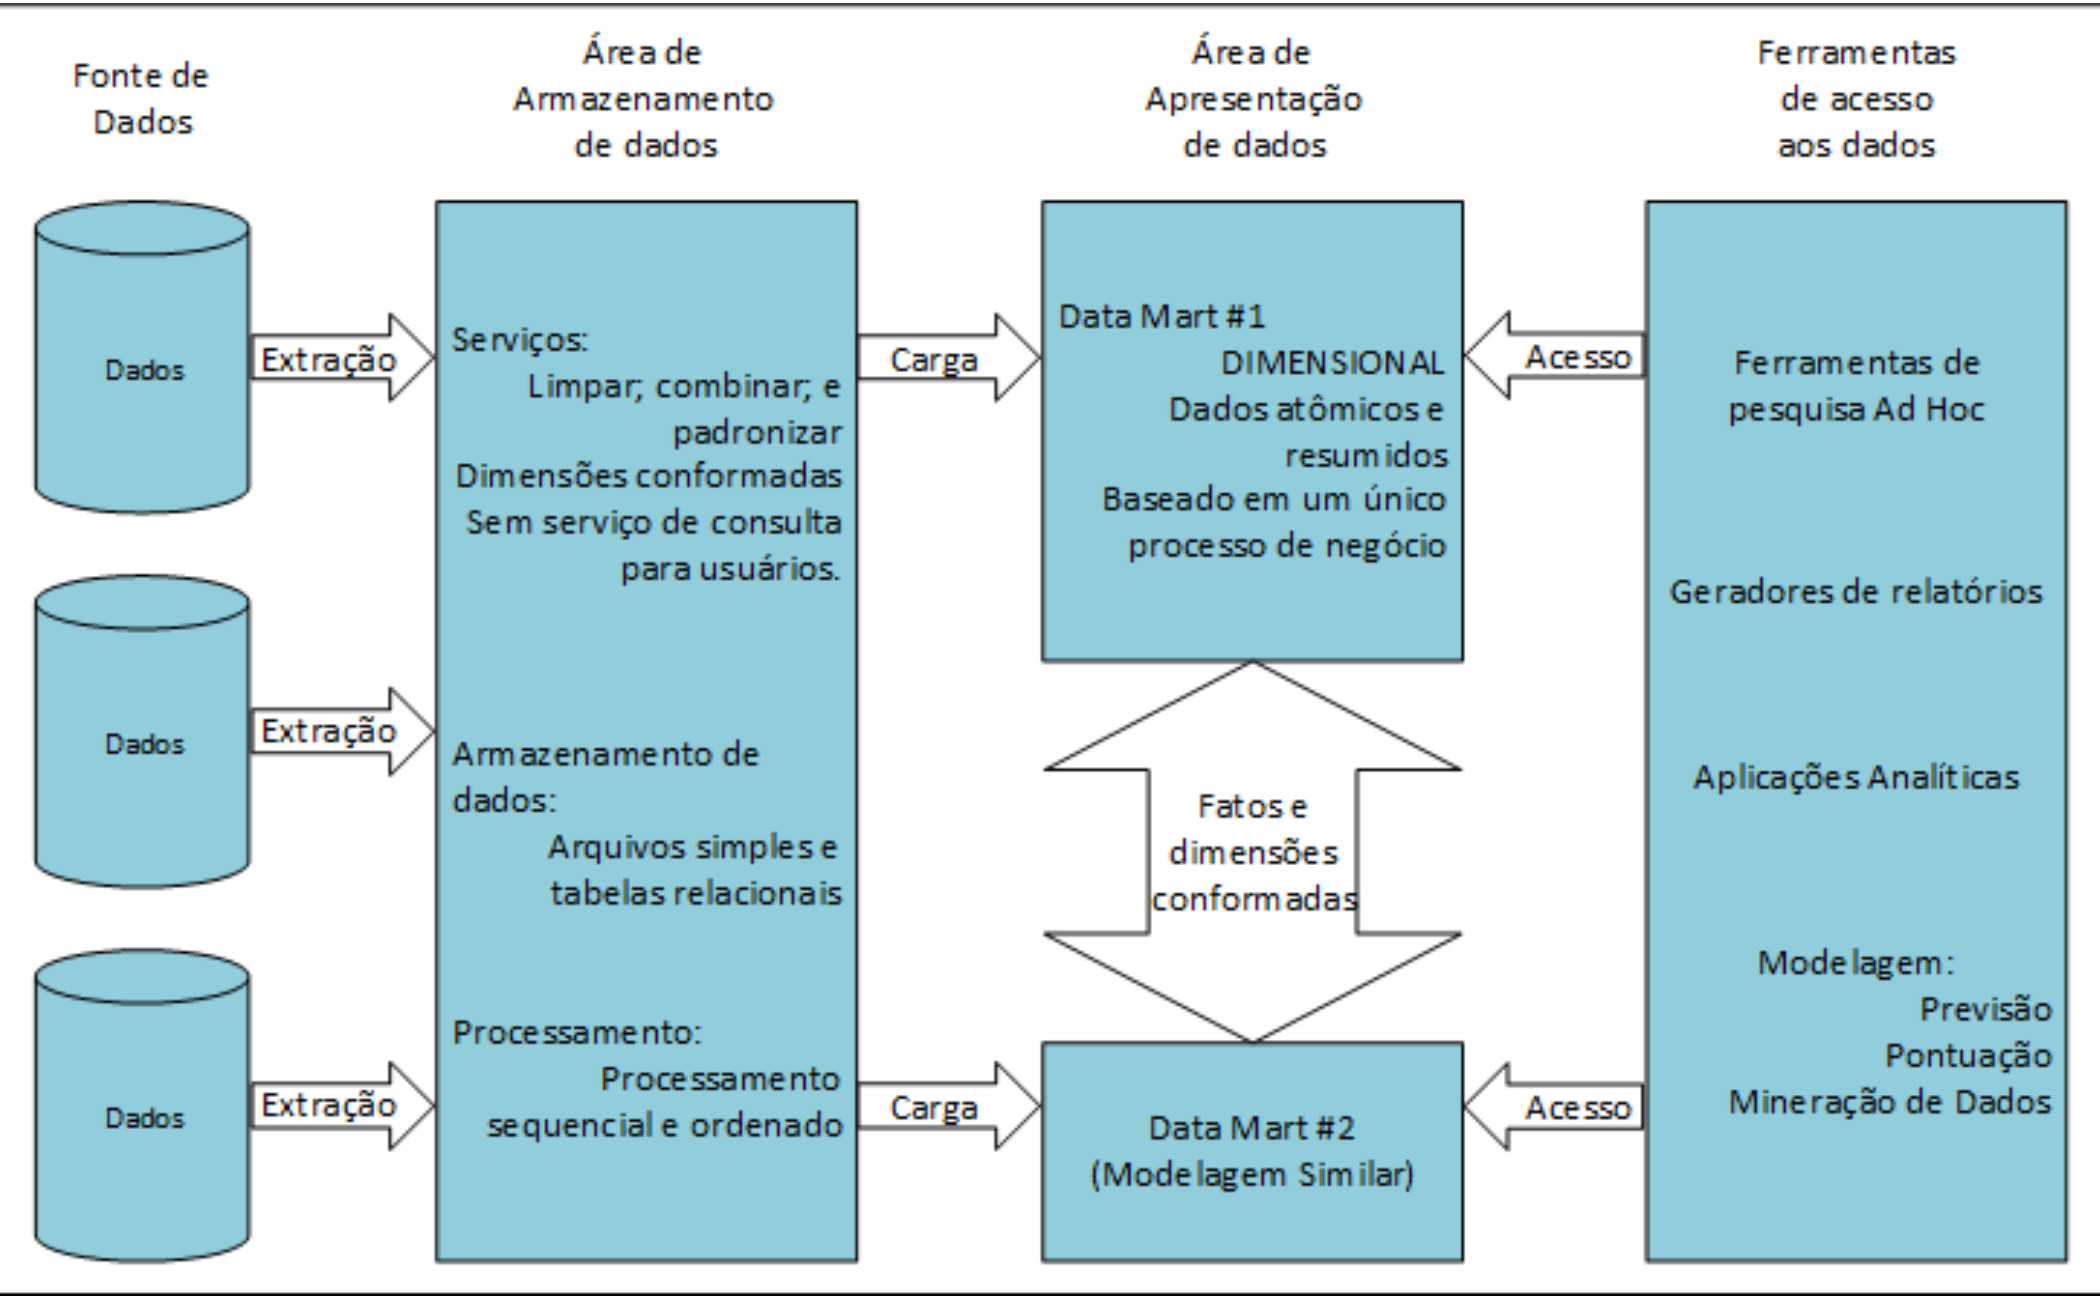
\includegraphics[scale=0.7]{figuras/DWcomponentes.png}
		\caption{Componentes de um DWing. Fonte \cite{kimball}}
		\label{componentesdw}
\end{figure}

\subsection{Sistemas de fonte de dados Operacionais}

O sistemas de fonte de dados Operacionais (OSS) são as fontes dos dados de negócio que irá compor o ambiente de DW. Pode ser de origem de várias aplicações que compõe o sistema corporativo de uma instituição, podendo ser unificada com uma única ou várias bases de dados.  Essas bases de dados não precisam ser necessariamente da mesma tecnologia, podendo ser um banco de dados transacionais, arquivos de texto, planilhas, arquivos xml ou qualquer outra forma de se armazenar e representar informações de negócio. As fontes de dados não podem ser consideradas dentro do escopo do DWing, pois  não se tem nenhum controle sobre o conteúdo ou sobre o formato de dados provenientes da fonte \cite{kimball2002}.

\subsection{Área de preparação dos dados}

A área de Preparação dos dados (DAS) é o ambiente na qual é feita a extração, transformação e carga dos dados operacionais, processo comumente chamado de ETL. Essa área de preparação, denominada por Kimball (\citeyear{kimball2002}), utiliza arquivos simples ou tabelas relacionais temporários, não acessíveis aos usuários, para armazenamento e manipulação das informações durante o processo de ETL. Assim que os dados estiverem prontos é feito a carga na base de dados dimensional, esta, acessível ao usuário.

%

A etapa de extração dos dados consiste em ler e entender as fontes de dados e extrair apenas os dados necessários para o DW. Os dados extraidos na camada OSS não são integrados, e, segundo Inmon (\citeyear{inmon2002}), esses dados, dessa forma, não podem ser utilizados para dar suporte a uma visão corporativa dos dados, que é uma das essências do ambiente de DWing. Dessa forma, uma série de transformações podem ser feitas buscando a limpeza de dados (resolução de conflitos, tratamento de informações não existente, conversão de dados para um formato padronizado), combinação de dados de diversas fontes, remoção de dados duplicados e atribuições de chaves que serão utilizadas no DW \cite{kimball2002}. Ao final da transformação, as informações necessárias são selecionadas e incluídas na base de dados multidimensional, encontrada na área de apresentação que será tratada em seguida.

\subsection{Área de apresentação}

A área de apresentação dos dados (DPA) é onde os dados são organizados, armazenados e disponibilizados para consultas á usuários ou ferramentas de geração de relatórios ou análises. Esse ambiente pode ser materializado no DW em si \cite{kimball2002}. 

%

Um dos propósitos de um DW é ter uma navegação intuitiva e de alta performance \cite{kimball2002}. A visualização das informações de um DW é resultado de agregações de dados, ou seja, diferentes formas de agrupamentos de dados que geram diferentes tipos de informações. Essas agregações são caracterizadas pelas consultas OLAP. Dessa forma, a modelagem relacional, normalmente utilizadas em bancos de dados transacionais, não dão suporte esses propósitos, pois a base de dados é normalizada e a agregação de grande número de dados torna-se custosa em termos de performance. O processo de normalização foi inicialmente proposto por Byce Codd  que consiste em esquematizar as relações de uma base de dados relacional, minimizando redundância de informações e anomalias de inserção, exclusão e alteração, no que diz respeito a manter a consistência de dados caso haja a duplicidade deste. Dessa forma, uma base de dados relacional normalizada oferece mais segurança em transações de acesso e alteração/inclusão/deleção de dados pois possui esquemas menores e consistentes \cite{elmasri2006}. O problema de esquemas menores é a performance, pois a realização consultas exige a navegação  entre várias tabelas, e se tratando de uma consulta que envolve grande quantidades de dados, como em um DWing, a performance se torna um fator muito importante para a qualidade do ambiente.

%

Kimball (\citeyear{kimball2002}) então propõe o uso da modelagem dimensional, que possui as mesmas informações que as bases normalizadas, porém em um formato diferente, atendendo a facilidade na navegação e na performance das consultas. Mais detalhamento sobre a modelagem dimensional será visto na Seção (\ref{sec-dimensional-modeling}).

%

\subsection{Ferramentas de Acesso de dados – Vizualização de dados}

%

As Ferramentas de acesso a dados são ferramentas que tem a capacidade de realizar consulta aos dados da Área de apresentação. Elas podem variar desde uma simples ferramentas de consulta ad hoc até ferramentas de análises complexas e de mineração de dados \cite{kimball2002}.

(COMPLETAR FALANDO SOBRE algumas formas de visualização: graficos, dashboards...)

%

\section{Modelage dimensional}
\label{sec-dimensional-modeling}

%

A modelagem dimensional é mais simples, mais expressiva e mais fácil de compreender do que a modelagem relacional \cite{ballard1998}. A modelagem dimensional busca obter um modelo que representa um conjunto de medidas que são descritas por aspectos comuns de negócio.

%

Os conceitos básicos da modelagem dimensional são:

\begin{itemize}
	\item \textbf{fatos}: são dados que contém medidas e seu contexto. Cada fato pode representar uma transação do negócio ou um evento que pode ser usado para análise do próprio negócio. São instâncias da realidade  que podem ser mensuradas de maneira quantitativa \cite{kiball2002}.Em um DW os fatos são armazenadas em tabelas de fatos, que consomem cerca de 90\% do espaço de uma base de dados dimensional. Tabela de fatos é a principal tabela de um modelo dimensional \cite{kimball2002} \cite{ballard1998}.
	\item \textbf{dimensões}: determinam os detalhes do contexto em que foi obtido um fato. São tabelas que contem as descrições textuais de negócio e ajudam na identificação de um componente da respectiva dimensão. Cada fato se relaciona com várias dimensões, associado a apenas a um dado em cada uma dessas dimensões.
	\item \textbf{medidas}: é um atributo numérico do fato. A medida determina a performance ou o comportamento de aspectos do negócio. As medidas são determinadas como combinações de membros de dimensões e alocados na tabela de fatos.
\end{itemize}

%

A idéia da modelagem dimensional é representar os tipos de dados de negócio em estruturas de cubo de dados. As células desse cubo contém os valores medidos e os lados definem as dimensões.

COLICAR IMAGEM DE CUBO

%

O modelo dimensional proposto por Kimball (\citeyear{kiball2002}) é chamado de star scheme. Nele, temos a tabela fato no centro e varias tabelas dimensões se relacionando com essa tabela fato. As tabelas fatos devem possuir duas ou mais chaves estrangeiras para as chaves primarias de diferentes dimensões. Para juntar as informações basta fazer o join entre elas.

COLOCAR IMAGEM DO ESQUEMA ESTRELA

%

Uma Tabela de dimensão deve ser construída de maneira a incluir atributos que podem ser agregados, fornecendo ao usuário maneiras alternativas de visualizar as as informações. Como por exemplo, uma tabela de produto tem o atributo “nome do produto” e o atributo “categoria”. Dessa forma, o usuário poderá agrupar os produtos por categoria para ter uma diferente visão sobre a informação. Diferente do modelo relacional, o fato da tabela dimensão não ser normalizada implica na melhoria da performance, pois nesse exemplo citado, “categoria” do produto normalmente seria outra tabela, e para a referida análise seria necessário a realização de um Join, que foi substituído apenas por uma clausula \emph{Group by}.

%

Porém, tabelas dimensões podem ser normalizadas com o intuito de diminuir o uso do espaço de armazenamento de informações redundantes \cite{kimball2002}. Nesse caso, quando uma dimensão é normalizada passa-se a ter o esquema floco de neve. Esse esquema torna mais fácil a manutenção de dimensões, porém é aconselhado o seu uso apenas em situações que realmente seja necessário abrir mão da performance que o esquema estrela oferece.

COLOCAR IMAGEM DO SNOW FLAck

%

A modelagem dimensional facilita o processamento analítico dos dados (OLAP), aspecto que será tratado na seção (\ref{sec-olap}).

%

 Kimbal (\citeyear{kimball2002}) define quatro passos que guiam o processo da modelagem dimensional, que são:

 %

 \begin{itemize}
 	\item \textbf{Selecionar o processo de negócio a ser modelado}: consiste em definir qual o assunto na qual o DWing será orientado. Como ja foi explicado, o DW é orientado a assunto, e tomando como exemplo um sistema de vendas de uma loja, pode ser feita a análise sobre as vendas, sobre o estoque, etc. Selecionar o processo de negócio é selecionar qual desses assuntos serão analizados e modelados.
 	\item \textbf{Declarar o \emph{"grão"} do processo de negócio}: significa especificar exatamente o que uma linha da tabela de fatos representa. Nessa etapa é definido o nível de glanuralidade da informação. Por exemplo, visualizar as informações por dia ou por mês. A granularidade se refere ao nível de detalhe que o fato deve ter. 
 	\item \textbf{Escolher as dimensões}: consiste em definir as dimensões que se aplicam acada linha de fato que foi definido. Se o nível granularidade foi bem definido, é fácil definir as dimensões. 
 	\item \textbf{Identificar fatos}: consite em responder a pergunta "	o que estamos medindo?". Nessa estapa é definido os fatos numéricos que irão popular as tabelas fatos.	  
 \end{itemize}

\section{OLAP}
\label{sec-olap}

%

O processamento analítico \emph{On-Line} (OLAP – \emph{On-line Analytc Processing}) é toda atividade de consulta que busca trazer ao usuário uma visão analítica dos dados através de comparações, visões personalizadas, análises históricas, diferentes cenários e entre outras opções \cite{kimball2002}. Pode-se definir OLAP como sistemas ou ferramentas que realizam consultas ao DW. Tais sistemas permitem aumentar ou diminuir o nível de detalhes da informação através das seguintes operações:

%

\begin{itemize}
\item \textbf{\emph{Drill down}}: Consiste em navegar em uma informação de menor nível de detalhe para uma informação de maior nível de detalhe. Por exemplo, uma análise utilizando a dimensão tempo fornece o tempo por ano. Uma operação de Drill Down consistiria e trazer essa mesma informação por mês.
\item \textbf{\emph{Roll up}}: Consiste em navegar em uma informação de maior nível de detalhe para um menor nível de detalhes. É exatamente o inverso do Drill down.
\item \textbf{\emph{Slice and dice}}: A operação de slice consiste em fatiar o cubo, que consiste em selecionar um atributo de uma dimensão específica e olhar apenas as informações das outras dimensões sobre esse atributo, eliminando a dimensão fatiada. Por exemplo, em um cubo com informações sobre a venda,  fatiar este cubo pelo ano 2012 consiste em eliminar a dimensão tempo e apenas considerar as vendas para o ano de 2012. A Operação dice, como o nome sugere, consiste em fatiar em formato de cubo. Nessa caso, não será eliminado nenhuma dimensão, mas será selecionado alguns subgrupos em duas ou mais dimensões, resultando em um subcubo. Por exemplo,  a operação de dice em um cubo de vendas consiste em selecionar as vendas entre o ano de 2010 a 2013, nas localizações “Rio de janeiro”, “São Paulo”, “Distrito Federal” e produtos de categoria “Alimentos” e “Eletronicos”.
\item \textbf{\emph{Pivoting}}: Também conhecida como \emph{rotate}, é uma operação que realiza uma rotação nos eixos de um cubo, gerando uma visualização alternativa da informação.[Cavalcanti, tiago]
\end{itemize}

%

\section{Ciclo de vida de um ambiente de \emph{Data Warehousing}}

%

Kimball (\citeyear{kimball2002}) define um ciclo de vida para o processo de construção de um ambiente de DWing. Neste ciclo, a primeira atividade a ser realizada é o planejamento do projeto. Essa atividade consiste em avaliar a iniciativa de construção do DWing, estabelecendo um escopo inicial e a justificativa, como também contempla a obtenção  de recursos e o lançamento do projeto.

(COLOCAR FIGURA DO CICLO DE VIDA)
%
%

A próxima atividade é a definição dos requisitos de negócio. O alinhamento do DWing com o s requisitos dos usuários é absolutamente crucial. Não adianta construir o ambiente com as melhores ferramentas do mercado se o este não fornece a informação que o usuário precisa ver. Dessa forma, mais de 50\% das iniciativas de DWing não tem sucesso \cite{sen2011}. Pelo levantamento feito na pesquisa de Kimpel (\citeyear{kimpel2013}), a principal causa é o não entendimento do problema que o usuário de negócio quer solucionar. E é na etapa de requistos que o problema e as necessidades devem ser entendidos e transformados em requistos de negócio para as etapas seguintes, de modelagem e construção do ambiente.

%

Com os requistos definidos, existem três conjuntos de tarefas. As tarefas superiores da figura (????) são responsaveis pela concepção tecnologica do ambiente. Consiste na definição da arquitetura técnica e  seleção das tecnologias envolvidas na solução de DWing. O conjunto de tarefas que se encontram no meio do ciclo são responsáveis pelo desenho do modelo dimensional, modelo físico e a definição e desenvolvimento do processo de ETL dos dados. O conjunto de tarefas inferiores são responáveis pelo desenho e desenvolvimento das aplicações analíticas, que irão fornecer a visualização da informação gerada pela DWing para o usuário. Juntando esses tres conjuntos de tarefas temos a implantação e disponibilização do ambiente de DWing para o usuário, então pode-se dizer que a solução de DWing foi implantada e pode começar a ser utilizada. 

%

No fim do ciclo ainda existe uma atividade de manutenção e crescimento do ambiente, dado que esse é um tipo de ambiente que deve evoluir dinamicamente de acordo com o negócio e suas necessidades de tomada de decisão.
